%%%%%%%%%%%%%%% Paigen's 28 array data %%%%%%%%%%%%%%%%%%%%%%%%
\newpage
\subsection{Paigen's 300-gene experiment}
This is a multiple factor 28-array experiment. 
The experiment is done in Beverly Paigen's Lab in The Jackson Lab. 
They took three strains of mice and feed them with two kind of 
diets. In that way you get six kind of mice. They picked two
individuals in each group then you have totally 12 distinct mice.
So in this experiment, you have strain, diet and biological replicates
as the factors. You can test the effects from any factor or
any combination of them. 
The experimental deign in shown in table \ref{tbl:paigen} 
and figure \ref{fig:paigen}. 

% table for mouse assignment
\begin{table}[htb]
\centering
\begin{tabular}{|l|c|c|} \hline
& Hi fat diet & Low fat diet\\
 \hline
Strain:Pera & A1, A2 & E1, E2\\ \hline
Strain:I & B1, B2 & F1, F2\\ \hline
Strain:DBA & C1, C2 & D1, D2\\ \hline
\end{tabular}
\caption{Mice used in Paigen's 28-array experiment}
\label{tbl:paigen}
\end{table}

% figure for expt design
\begin{figure}[htbp]
\centering
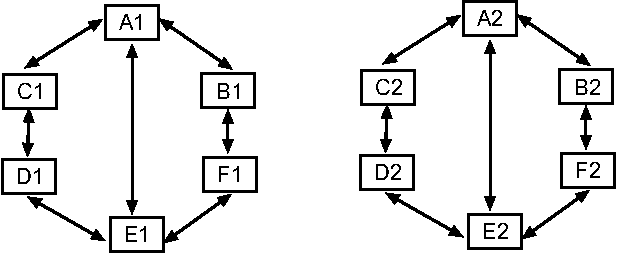
\includegraphics{paigen}
\caption{Array assignment in Paigen's 28-array experiment}
\label{fig:paigen}
\end{figure}

We will skip the data quality check
and transformation steps in this example.
We will show you how to test different terms in the model
in a multiple factor design. In this design, there are strain
effect, diet effect, strain by diet interaction effect and
biological replicate effect. The interaction effect is nested
within the biological replicate effect.

\begin{enumerate}
\item Load in data 
\begin{Sinput}
R> data(paigen)
\end{Sinput}

\item Make data object with replicates collapsed. Note that
if we donot collapse replicates, we need to put Spot in the 
model as a random terms. That will make the calculation 
even slower. Based on our experience, collapsing replicates
gives similar results as not collapsing and fit Spot effect
as random.
\begin{Sinput}
R> paigen <- createData(rawdata, 2, 1)
\end{Sinput}

\item Make several model object and fit ANOVA. 
First make full model object with Strain, Diet, 
interaction and biological replicate effects.
\begin{Sinput}
R> model.full.mix <- makeModel(data=paigen,
     formula=~Dye+Array+Strain+Diet+Strain:Diet,
     random=~Array+Sample)
R> anova.full.mix <- fitmaanova(paigen, model.full.mix)
\end{Sinput}
We can do a variance component plot on ANOVA result.
\begin{Sinput}
R> varplot(anova.full.mix)
\end{Sinput}
Then make a model object without interaction effect and fit ANOVA model
\begin{Sinput}
R> model.noint.mix <- makeModel(data=paigen, 
   formula=~Dye+Array+Strain+Diet+Sample, random=~Array+Sample)
R> anova.noint.mix <- fitmaanova(paigen, model.noint.mix)
\end{Sinput}

\item F test on different effects. 
First we want to test the interaction effect. 
The interaction effect must be tested in the full model. Note that because the
interaction effect is nested within biological replicates, we have to use
biorep to test the interaction.
\begin{Sinput}
R> ftest.int.mix <- matest(data=paigen, model=model.full.mix, 
          term="Strain:Diet")
R> idx.int.mix <- volcano(anova.full.mix, ftest.int.mix)
\end{Sinput}
Then we want to test the Strain and Diet effect. 
We use the model without interaction
to test the main effect.
\begin{Sinput}
R> ftest.strain.mix <- matest(data=paigen, model=model.noint.mix, 
          term="Strain")
R> ftest.diet.mix <- matest(data=paigen, model=model.noint.mix, 
          term="Diet")
\end{Sinput}
We can do volcano plot to visualize the F-test results and pick significant
genes. That step is skipped here.

\item Now we can do T-test on any comparison on a given term. 
The result still contains the F values (with numerator's degree of freedom
equals 1). To to do all pairwise comparison on Strain, first make
a comparison matrix:
\begin{Sinput}
R> C <- matrix(c(1,-1,0,1,0,-1, 0,1,-1), nrow=3, byrow=T)
\end{Sinput}
Users need to be careful about specifing comparsion matrix. The comparison
need to be the linear combination of the rows of the design matrix
for fixed terms. Otherwise the comparision will be non-estimable.

To do the test:
\begin{Sinput}
R> ttest.strain <- matest(paigen, model.noint.mix, term="Strain",
           Contrast=C, n.perm=500)
\end{Sinput}
Because we have three comparisons here, doing volcano will 
generate three plots.
\begin{Sinput}
R> volcano(ttest.strain)
\end{Sinput}

\end{enumerate}

Again, the clustering analysis is skipped here.


